\begin{figure}[H]
\centering
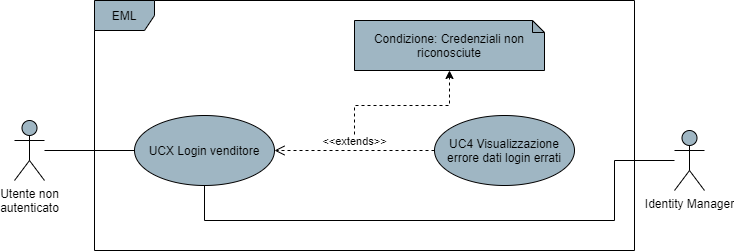
\includegraphics[scale=0.6]{res/UseCase/Immagini/LoginVenditore}
\caption{Schema generale: modulo di login venditore}
\end{figure}

\subsubsection{UCX - Login venditore}
\begin{itemize}
\item \textbf{Attori primari}: utente non autenticato;
\item \textbf{Attori secondari}: identity manager;
\item \textbf{Descrizione}: il venditore, inserendo le proprie credenziali, viene autenticato alla piattaforma;
\item \textbf{Scenario Principale}: l'utente non ancora autenticato accede alla pagina di login per il venditore, cliccando sul pulsante dedicato all'accesso alla merchant dashboard. Inserisce poi le proprie credenziali \textbf{[UCX.1]} e richiede il login \textbf{[UCX.2]};;
\item \textbf{Estensioni}:
\begin{itemize}
	\item \textbf{UC4}: se le credenziali inserite non vengono riconosciute dall'identity manager, viene visualizzato un messaggio che informa l'utente dell'errore;
\end{itemize}
\item \textbf{Precondizione}: il venditore prova ad autenticarsi alla piattaforma;
\item \textbf{Postcondizione}: il venditore viene autenticato e accede alla merchant dashboard.
\end{itemize}

\begin{figure}[H]
\centering
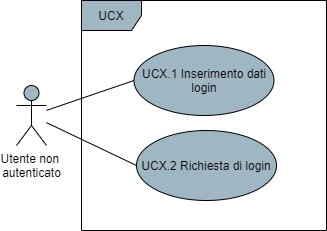
\includegraphics[scale=0.6]{res/UseCase/Immagini/LoginVenditoreSottocasi}
\caption{Diagramma UML\ped{G} per UCX - Login venditore}
\end{figure}

\subsubsection{UCX.1 - Inserimento dati login}
\begin{itemize}
\item \textbf{Attori primari}: utente non autenticato;
\item \textbf{Descrizione}: il venditore compila il form per il login;
\item \textbf{Scenario Principale}: l'utente inserisce nel form apposito i dati necessari al login.
\item \textbf{Precondizione}: il form di inserimento dati per il login è disponibile;
\item \textbf{Postcondizione}: i dati necessari al login sono stati compilati.
\end{itemize}

\subsubsection{UCX.1.1 - Inserimento password}
\begin{itemize}
\item \textbf{Attori primari}: utente non autenticato;
\item \textbf{Descrizione}: il venditore deve compilare il campo "Password" per procedere al login;
\item \textbf{Scenario Principale}: l'utente inserisce la sua password nell'apposito campo;
\item \textbf{Precondizione}: il campo "Password" risulta vuoto;
\item \textbf{Postcondizione}: il campo "Password" è stato compilato.
\end{itemize}

\subsubsection{UCX.1.2 - Inserimento email}
\begin{itemize}
\item \textbf{Attori primari}: utente non autenticato;
\item \textbf{Descrizione}: il venditore deve compilare il campo "Email" per procedere al login;
\item \textbf{Scenario Principale}: l'utente inserisce il suo indirizzo email nell'apposito campo;
\item \textbf{Precondizione}: il campo "Email" risulta vuoto;
\item \textbf{Postcondizione}: il campo "Email" è stato compilato.
\end{itemize}

\subsubsection{UCX.2 - Richiesta di login}
\begin{itemize}
\item \textbf{Attori primari}: utente non autenticato;
\item \textbf{Descrizione}: il venditore richiede l'autenticazione con i dati inseriti;
\item \textbf{Scenario Principale}: l'utente preme il tasto di login e manda la richiesta al sistema con i dati presenti nel form;
\item \textbf{Precondizione}: il venditore prova ad autenticarsi alla piattaforma;
\item \textbf{Postcondizione}: la richiesta di login è stata mandata al sistema.
\end{itemize} 